\section{MOOCs}

%-----------------------    ---------------------------------

\begin{frame}
\frametitle{¿Qué son los MOOCs?}

\begin{itemize}
   \item Cursos por Internet
   \item Hay algunos muy buenos, generalmente en inglés
   \item Generalmente gratis (algunos cobran por certificado, si lo terminas)
   \item Muchos de ellos ofrecidos por instituciones de renombre
   \item Basados generalmente en vídeos, lecturas y entrega de ejercicios
   \item Hay de todo: tecnológicos, de economía, de programación...
\end{itemize}

\end{frame}


%-----------------------    ---------------------------------

\begin{frame}
\frametitle{Sitios de MOOCs}

\begin{center}
  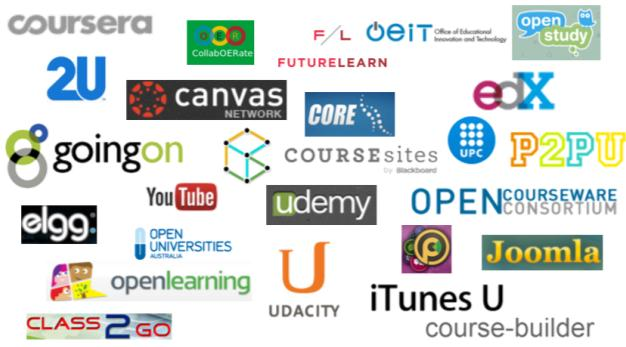
\includegraphics[width=10cm]{figs/sitios.jpg}
\end{center}


\begin{flushright}
{\tiny
Source: http://www.vocal.ie/wp-content/uploads/2014/06/MOOCs-Daigram11.jpg
}
\end{flushright}

\end{frame}

%-----------------------    ---------------------------------

\begin{frame}
\frametitle{Plataformas recomendadas}

\begin{itemize}
   \item Coursera (existe la aplicación CourseraCast para ver los vídeos con el Chromecast en la TV)
   \item edX: del MIT
   \item Udacity: spin-off de Univ. Stanford
   \item MiríadaX (en español)
\end{itemize}

\end{frame}



